\section{Fabricação}

\begin{frame}

    Substrato: N\textsuperscript{+}

    \begin{figure}[!htbp]
        \centering
        \caption{Formação das regiões N-drift, P\textsuperscript{+} e JFET}
        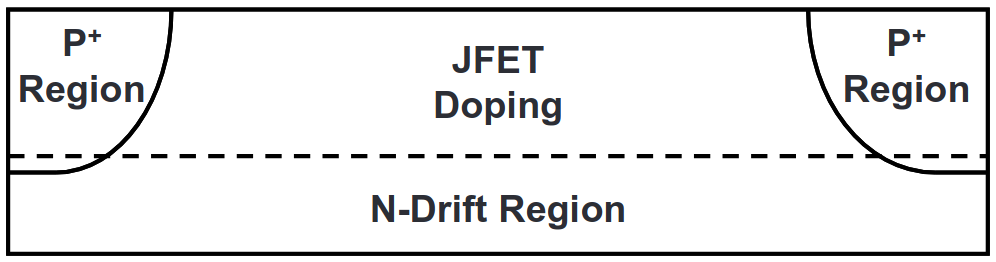
\includegraphics[scale=0.2]{imagens/dmos_fab_a.png}
        \\\small{\textbf{Fonte:} \cite{baliga2010fundamentals}}%
    \end{figure}

\end{frame}

\begin{frame}

    \begin{figure}[!htbp]
        \centering
        \caption{Deposição do eletrodo e dielétrico de \textit{gate}}
        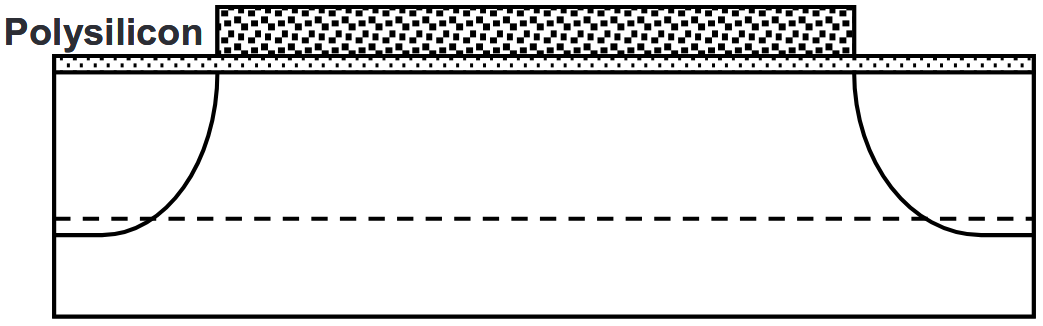
\includegraphics[scale=0.2]{imagens/dmos_fab_b.png}
        \\\small{\textbf{Fonte:} \cite{baliga2010fundamentals}}%
    \end{figure}

\end{frame}

\begin{frame}

    \begin{figure}[!htbp]
        \centering
        \caption{Formação da região P-base com o eletrodo de porta como mascara}
        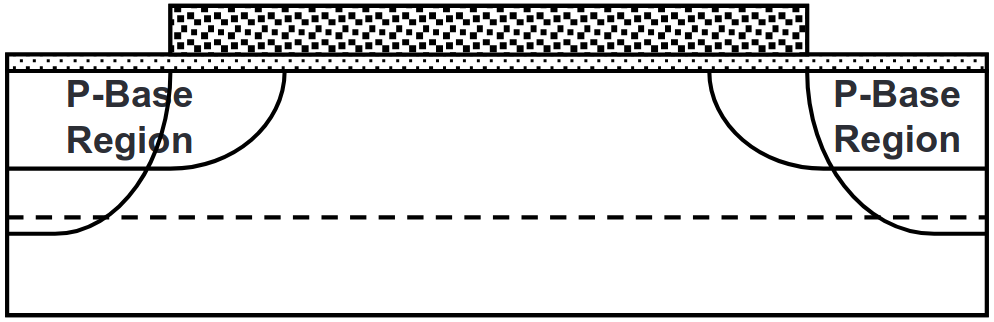
\includegraphics[scale=0.2]{imagens/dmos_fab_c.png}
        \\\small{\textbf{Fonte:} \cite{baliga2010fundamentals}}%
    \end{figure}

\end{frame}

\begin{frame}

    \begin{figure}[!htbp]
        \centering
        \caption{Formação da região de fonte controlada por fotoresistes laterais}
        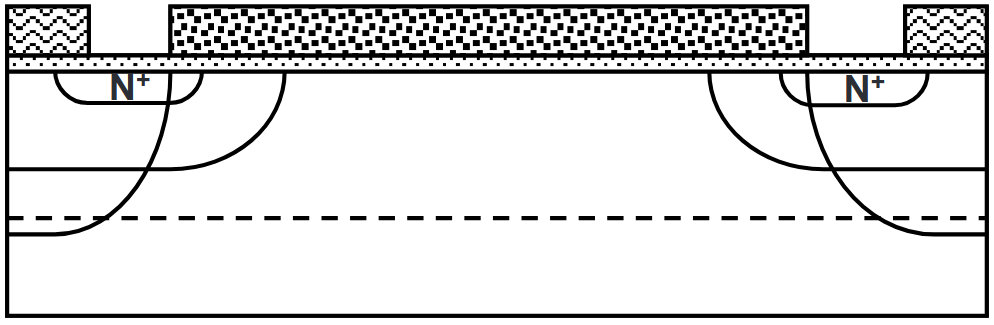
\includegraphics[scale=0.2]{imagens/dmos_fab_d.png}
        \\\small{\textbf{Fonte:} \cite{baliga2010fundamentals}}%
    \end{figure}

\end{frame}

\begin{frame}

    \begin{figure}[!htbp]
        \centering
        \caption{Deposição do dielétrico que separa porta e fonte}
        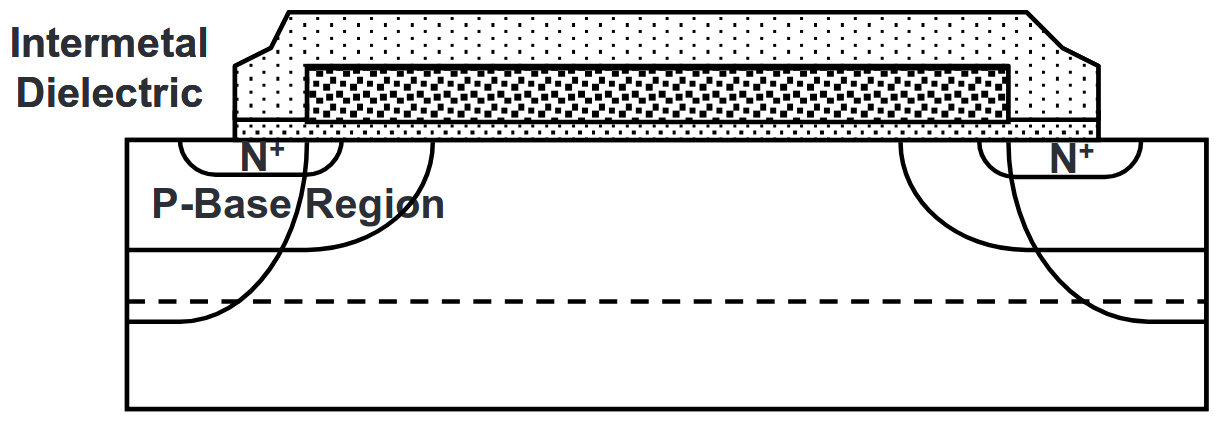
\includegraphics[scale=0.2]{imagens/dmos_fab_e.png}
        \\\small{\textbf{Fonte:} \cite{baliga2010fundamentals}}%
    \end{figure}

\end{frame}

\begin{frame}

    \begin{figure}[!htbp]
        \centering
        \caption{Deposição do metal de contato da fonte}
        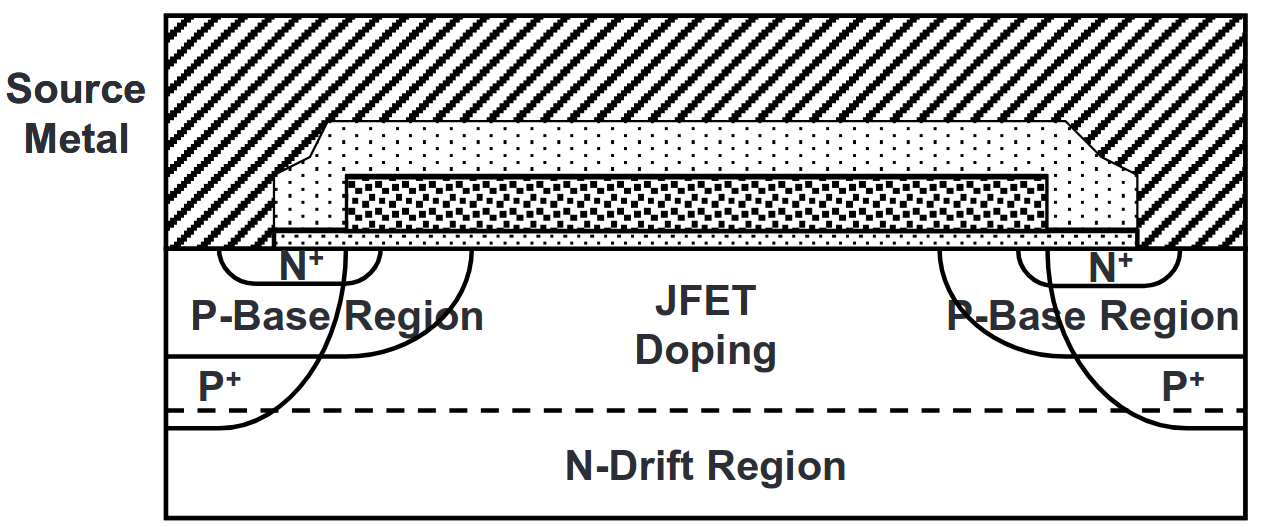
\includegraphics[scale=0.2]{imagens/dmos_fab_f.png}
        \\\small{\textbf{Fonte:} \cite{baliga2010fundamentals}}%
    \end{figure}

\end{frame}
